
\chapter {Installing and Setting Up Oscad}
\label{chap2}
The step by step instructions to install Oscad are given below.\\
Before starting the installation, please make sure that all the system and installation requirements and prerequisites are met. Installation script for Oscad is written in Bash.
This makes the installation efficient and user friendly.  \\
\newline
\textbf{System Requirements}
\begin{itemize}
\item Ubuntu 12.04 OS (64-bit/32-bit)\index{Ubuntu}
\item Oscad
\item Scilab 5.4.1
\end{itemize}
\textbf{Installation Requirements}
\begin{itemize}
\item Working Internet connection
\item Require to be an admin user to do the installation
\end{itemize}
\textbf{Prerequisites}
\begin{itemize}
\item Basic knowledge of analog and digital electronics
\item Basic knowledge of Linux shell commands\index{Linux}
\item Requires Synaptic Package Manager
\end{itemize}
%%%%%%%%%%%%%%%%%%%%%%
\shadowbox{Note: The Linux commands typed on Terminal during installation are given in boxes with round corners} 
%%%%%%%%%%%%%%%%%%%%%%%
\section {Procedure for installing Oscad}
\begin{itemize}
\item \textbf{Step 1: Download Oscad and examples} 

Go to \textbf{http://www.oscad.net/downloads}. Figure \ref{fig: Oscad Website} shows the downloads page of Oscad website.\\
\end{itemize}

\begin{figure}[h]
\centering
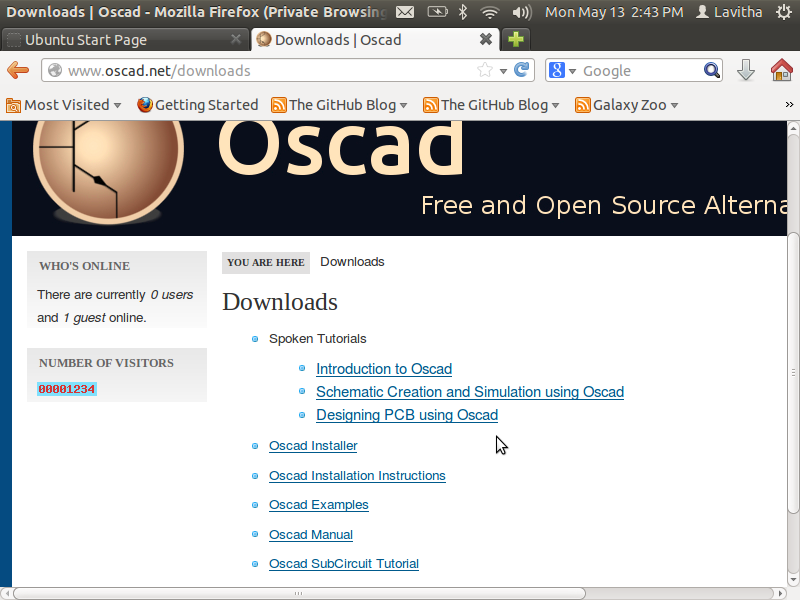
\includegraphics[width=0.7\textwidth]{figures/oscad1.png}
\caption{Oscad Website}
\label{fig: Oscad Website}
\end{figure}
\begin{enumerate}
\item Click on \textbf{Oscad Installer} and save the file in a folder\index{Oscad Installer}
\item Click on \textbf{Oscad Examples} and save the file in the same folder as above
\end{enumerate}
%%%%%%%%%%%%%%%%%%%%%%%%%%%%


%%%%%%%%%%%%%%%%%%%
\begin{itemize}
\item{\textbf{Step 2: Download Scilab }}\\
Go to \textbf{http://www.scilab.org/}. Click on the {\tt Download Scilab} option on the home page. Save the file in the same folder where Oscad installer and Examples were saved. Figure \ref{scilab} shows the Download Scilab option in the Scilab webpage.
\end{itemize}
%\newline
\shadowbox{Note: You can skip this step, if you have scilab 5.4.0 or above in your system}
\begin{figure}[h!]
\centering
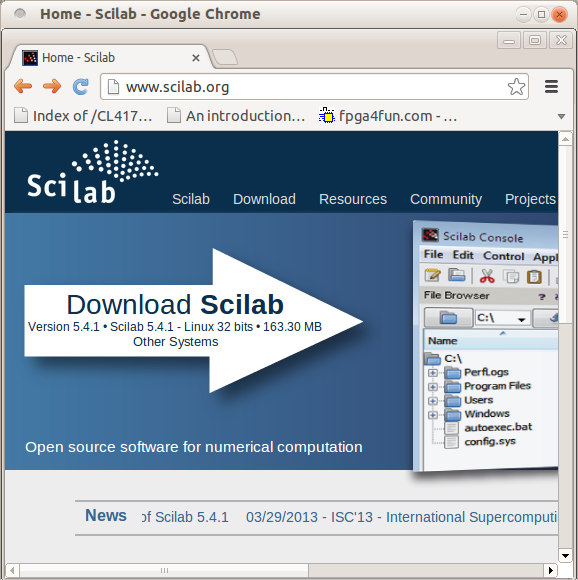
\includegraphics[width=0.5\textwidth]{figures/scilab.png}
\caption{Scilab website}
\label{scilab}
\end{figure}
%%%%%%%%%%%%%%%%%%%%%%%%%%
\newpage
\begin{itemize}
\item{\textbf{Step 3: Extract the downloaded files }}\\
Go to the folder where all the three files are saved. Select all, right click and choose \textbf{extract here} as shown in Figure \ref{extract}.
\end{itemize}
\begin{figure}[h!]
\centering
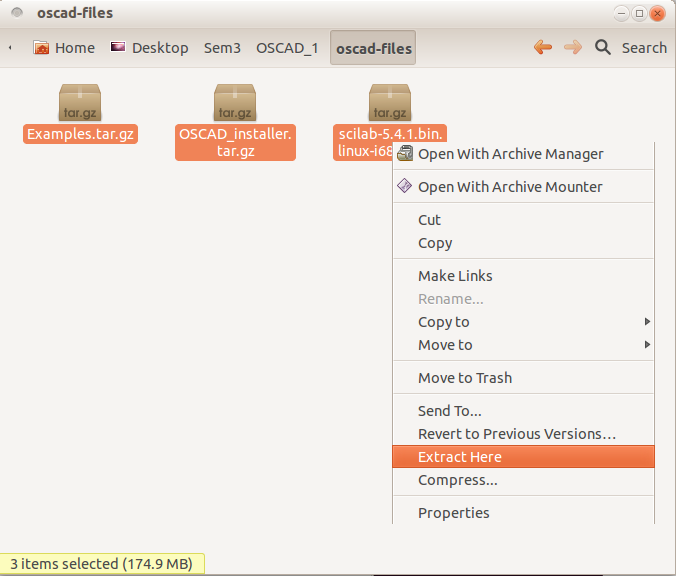
\includegraphics[width=0.9\textwidth]{figures/extract.png}
\caption{Extracting all files}
\label{extract}
\end{figure}
%%%%%%%%%%%%%%%%%%%%%%%%%%%
\begin{itemize}
\item{\textbf{Step 4: Navigate to Folder}}

Go to the directory where all the three folders are saved and extracted.\\
For this open a terminal window and type:\\
%\newline
\Ovalbox{\textbf{cd $<<$folder-where-downloaded-files-are-saved$>>$}}\\ In the above command, replace $folder-where-downloaded-files-are-saved$ with the path of the folder where you have saved and extracted the downloaded files.
Press Enter.\\
%\newline
Now check whether we have navigted to desired folder. To check please type:\\
\Ovalbox{\textbf{ls}}\\
Press Enter


Screen shot \ref{Terminalc} shows navigation to the folder having all files.
\end{itemize}
\begin{figure}[h!]
\centering
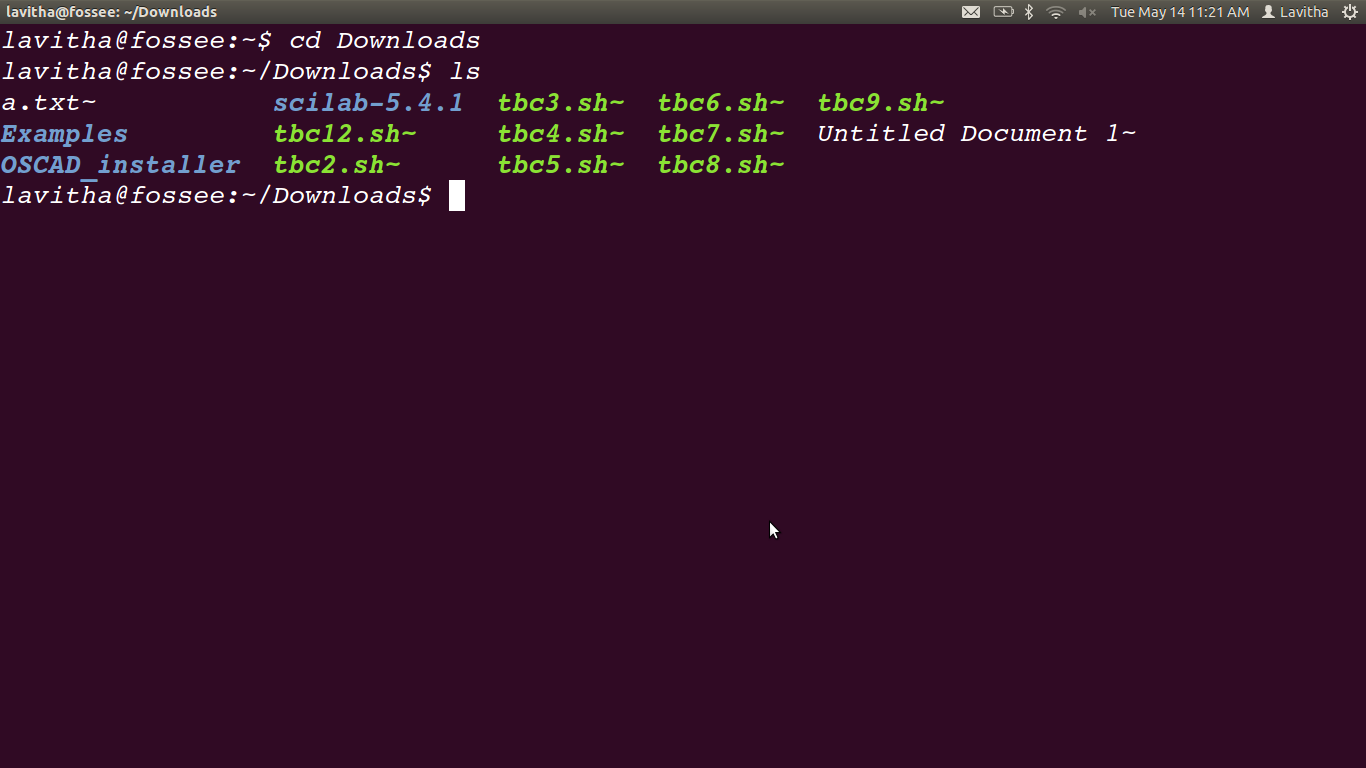
\includegraphics[width=0.9\textwidth]{figures/install0.png}
\caption{Terminal: Navigation to folder with required files}
\label{Terminalc}
\end{figure}
%%%%%%%%%%%%%%%%%%%%%%%%%%%%%%
\newpage
\begin{itemize}
\item{\textbf{Step 5: Navigate to OSCAD\_Installer}}\\
Now navigate to the folder {\tt OSCAD\_installer}. To do this type:\\
%\newline
\Ovalbox{\textbf{cd OSCAD\_installer}}\\
Press Enter
\newline
Figure \ref{termn} shows that we have navigated to OSCAD\_installer folder.
\end{itemize}
\begin{figure}[h!]
\centering
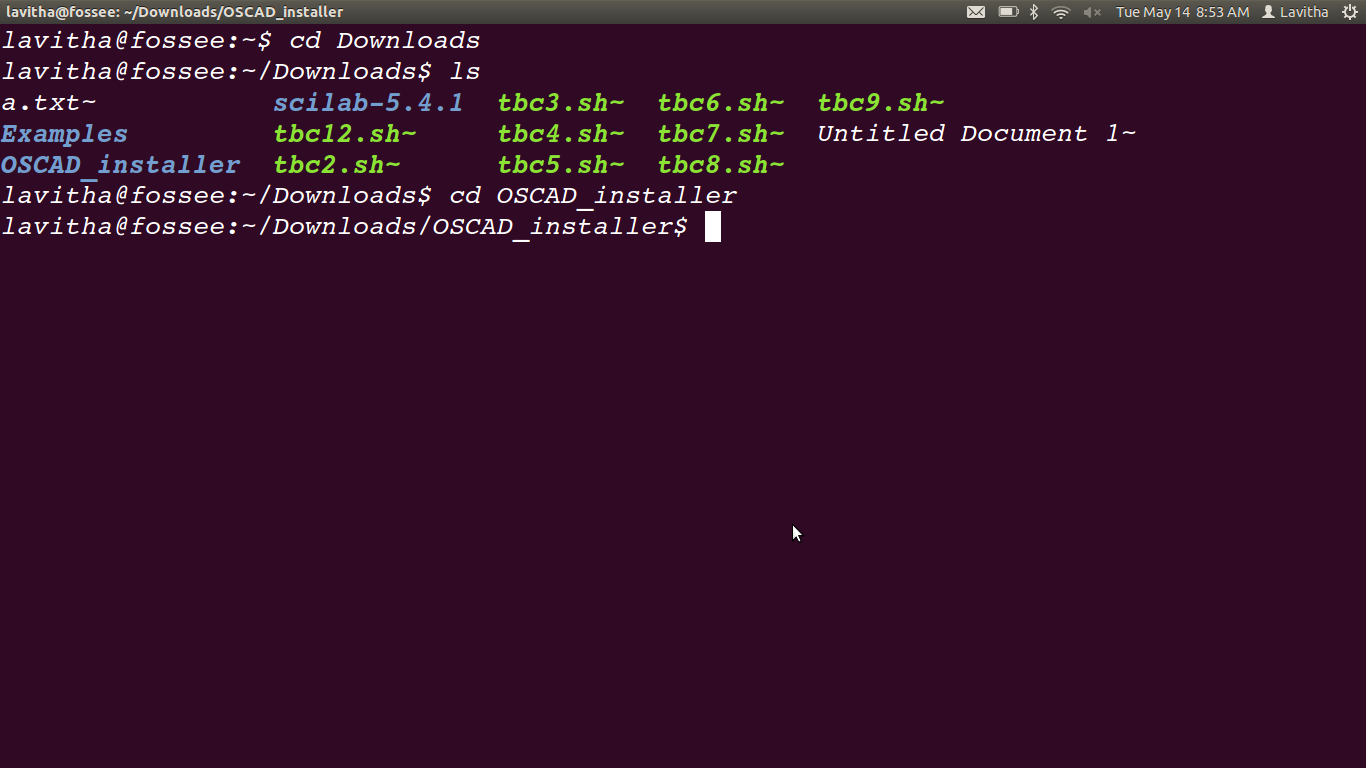
\includegraphics[width=0.9\textwidth]{figures/installer1.png}
\caption{Terminal: navigation to OSCAD\_installer}
\label{termn}
\end{figure}
%installer1.png

%%%%%%%%%%%%%%%%%%%%%%%%%%%%%%%%%%%%%
\begin{itemize}
\item{\textbf{Step 6: Make the installOSCAD and installModule files executable }}\index{installOSCAD.sh}\\
To do this go to terminal and Type:\\
\newline
\Ovalbox{\textbf{sudo chmod 755 installOSCAD.sh installModule.sh}}\\\\\index{installModule.sh}
Press Enter. 
Type the sudo (root) password. 
The Terminal should look like as shown in figure \ref{term}\index{Terminal}.
\end{itemize}
\newpage
\begin{figure}[h!]
\centering
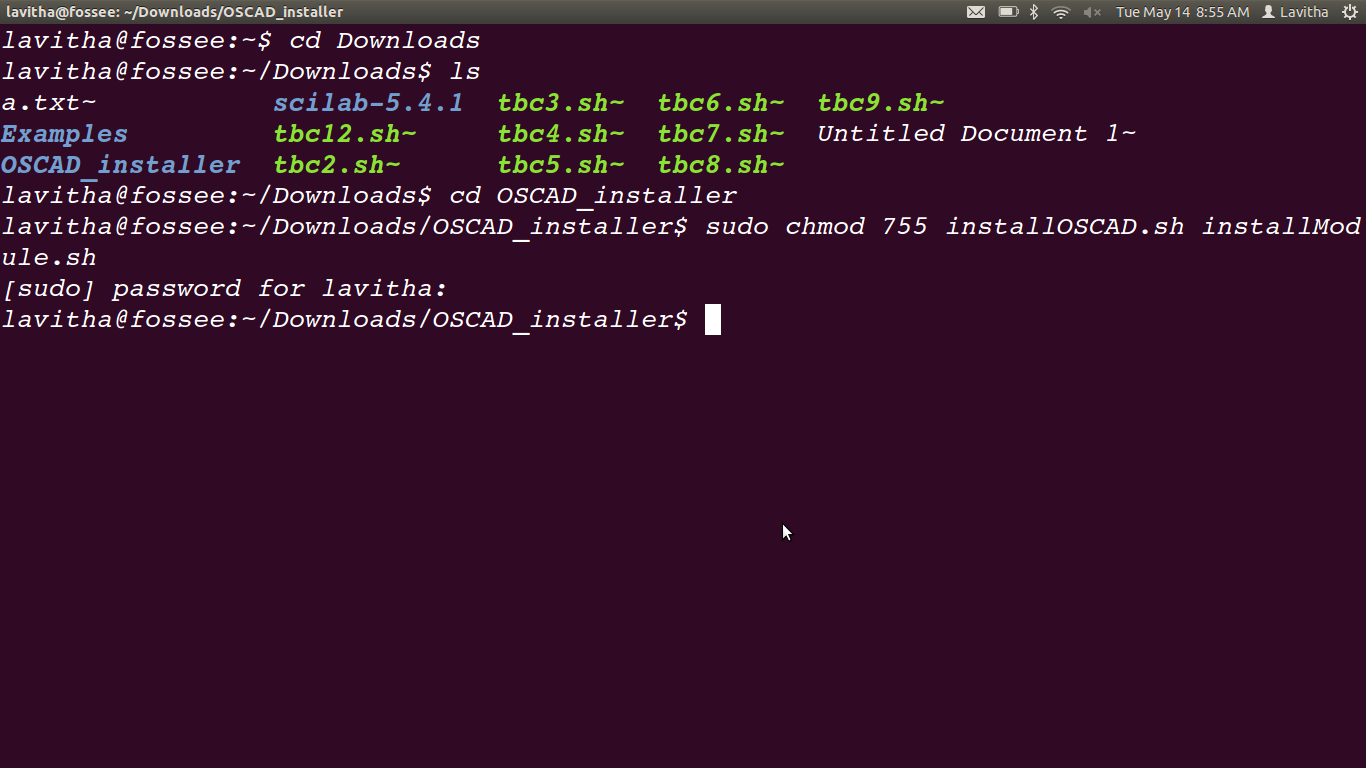
\includegraphics[width=0.9\textwidth]{figures/install3.png}
\caption{Terminal: make files executable}
\label{term}
\end{figure}
%%%%%%%%%%%%%%%%%%%%%%%%%%%%%%%%%%%%%%%%%%%%%
\begin{itemize}
\item{\textbf{Step 7: Begin installation }}
To begin installation, type\\
\newline
\Ovalbox{\textbf{ ./installOscad.sh}}\\
Press Enter\\
\newline
The Terminal prompts for proxy settings as shown in Figure \ref{proxy} \\\index{proxy}
\shadowbox{\textbf{Note: If you are not behind proxy type 'n' and press Enter.}}\\
\shadowbox{\textbf{You will not get the option to enter proxy parameters.}}
\newline
\begin{figure}[h!]
\centering
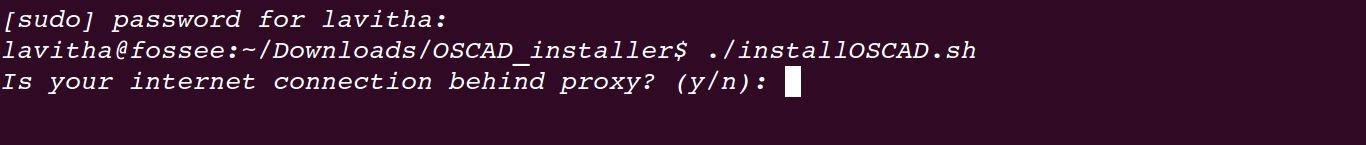
\includegraphics[width=0.9\textwidth]{figures/install4.png}
\caption{Terminal: Installation - Proxy settings}
\label{proxy}
\end{figure}\\
\newpage
If you typed `y', then enter the proxy details as shown in figure \ref{proxys}
\begin{figure}[h]
\centering
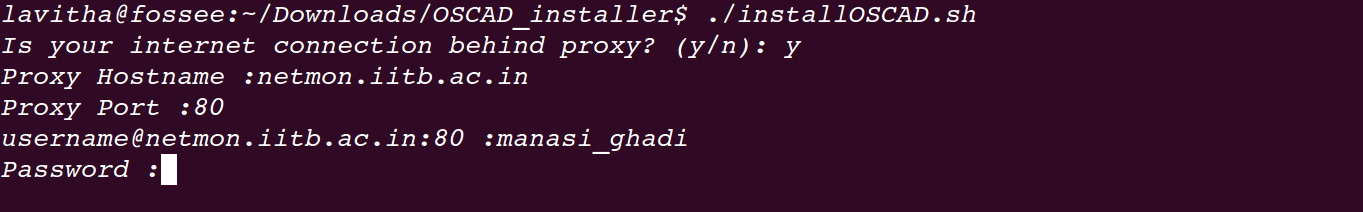
\includegraphics[width=0.9\textwidth]{figures/install5.png}
\caption{Terminal: Proxy}
\label{proxys}
\end{figure}
\newline
Now the prompt displays message 
\textbf{Do you want to continue [Y/n]:}\\
Type 'y' and press Enter. KiCad, Ngspice and necessary python modules will be installed.\\
\newline
\shadowbox{\textbf{Note: While installing the python modules, you may get some error messages}}\index{python}
\shadowbox{\textbf{In that case, install the missing packages using Synaptic Package Manager}}
\shadowbox{\textbf{Once this is done, re-run the installOscad.sh script.}}
\end{itemize}
%%%%%%%%%%%%%%%%%%%%%%%%%%%%%%%%%%%%%%
\begin{itemize}
\item{\textbf{Step 8: Linking of Scilab}}
The prompt displays the message:\\
\textbf{Do you have scilab 5.4 or above? (y/n)} as shown in figure \ref{link}
\begin{figure}[h]
\centering
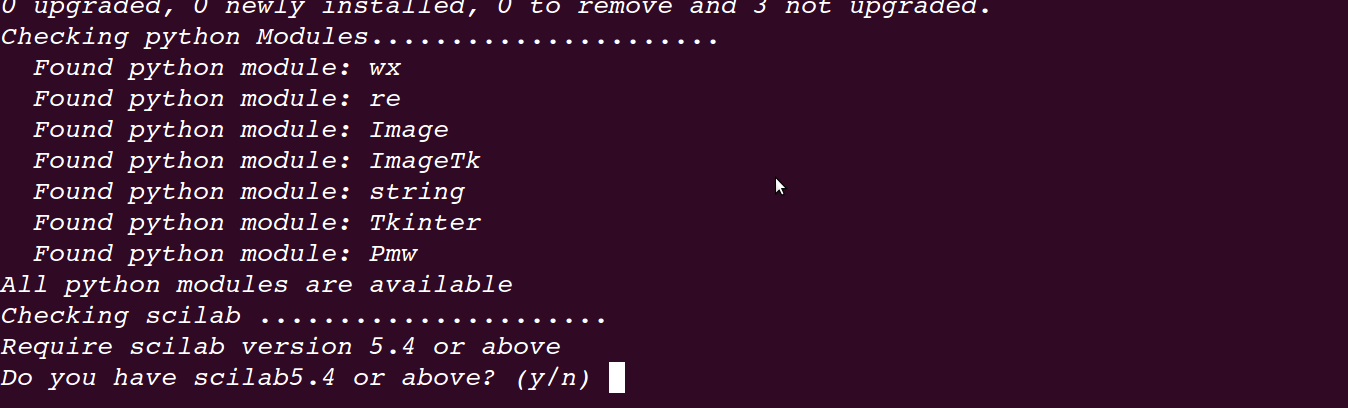
\includegraphics[width=0.9\textwidth]{figures/install6.png}
\caption{Terminal: Linking Scilab}
\label{link}
\end{figure}
\newpage
Type 'y' and press Enter. Now give the complete path where you have saved Scilab 5.4.0 or above.\\
\newline
Example:\\
\textbf{\Ovalbox{/home/lavitha/downloads/scilab-5.4.1}}\\
\newline
Press Enter. 
The screen shot is shown in figure \ref{path}\\
\newline
\begin{figure}[h]
\centering
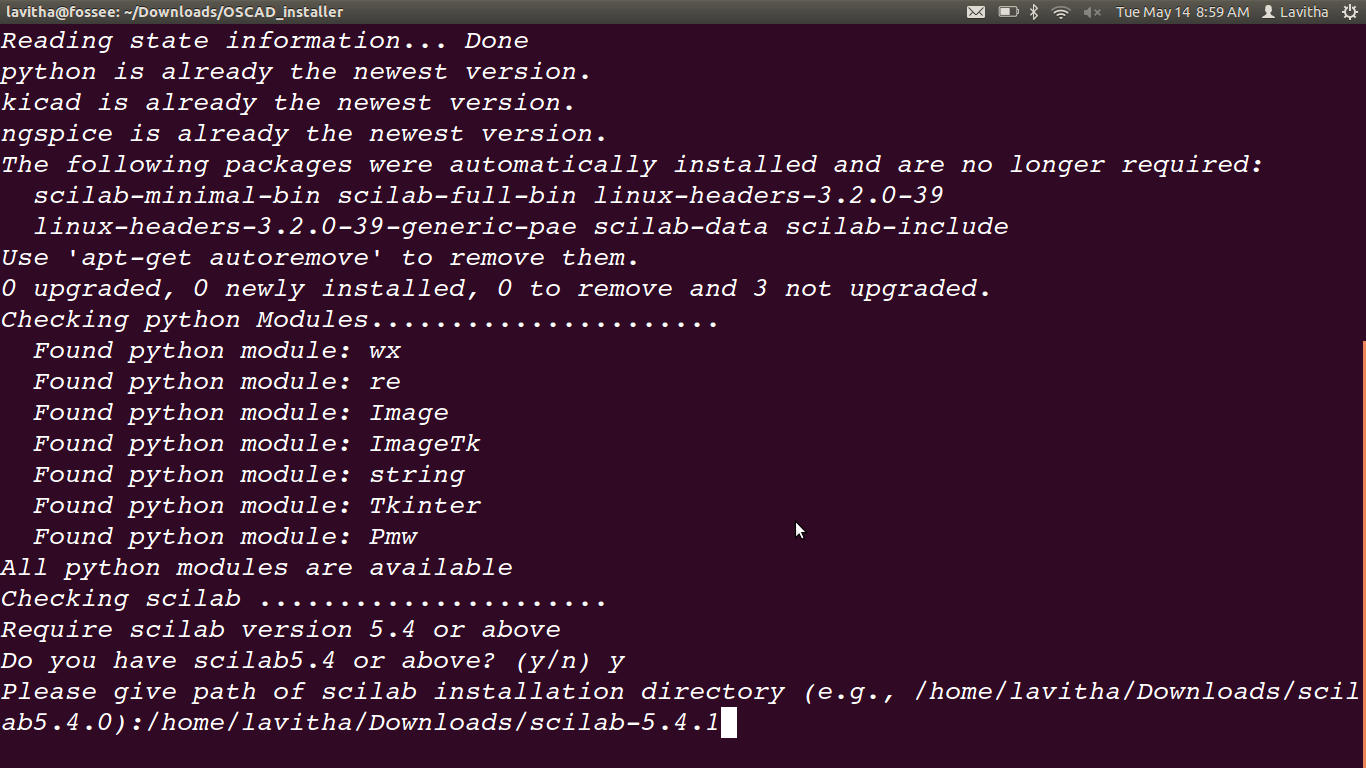
\includegraphics[width=0.9\textwidth]{figures/install7.png}
\caption{Terminal: Scilab instllation}
\label{path}
\end{figure}
\shadowbox{\textbf{Note: The \textbf{metanet library} will be installed after this step. It takes a couple of minutes}}
\end{itemize}
%%%%%%%%%%%%%%%%%%%%%%%
\begin{itemize}
\item{\textbf{Step 9: Final installation}}
The prompt displays the message
\textbf{Please select installation directory}\\
Type the desired location where you want to install Oscad.\\
\newline
For example:\\
\Ovalbox{\textbf{/home/lavitha}}\\
Press Enter\\
\newline
If everything is installed then the message\\
\textbf{installation completed} is displayed as shown in screen shot \ref{installi}. This creates \textbf{Oscad} shortcut on Desktop.
\end{itemize}
\begin{figure}[h]
\centering
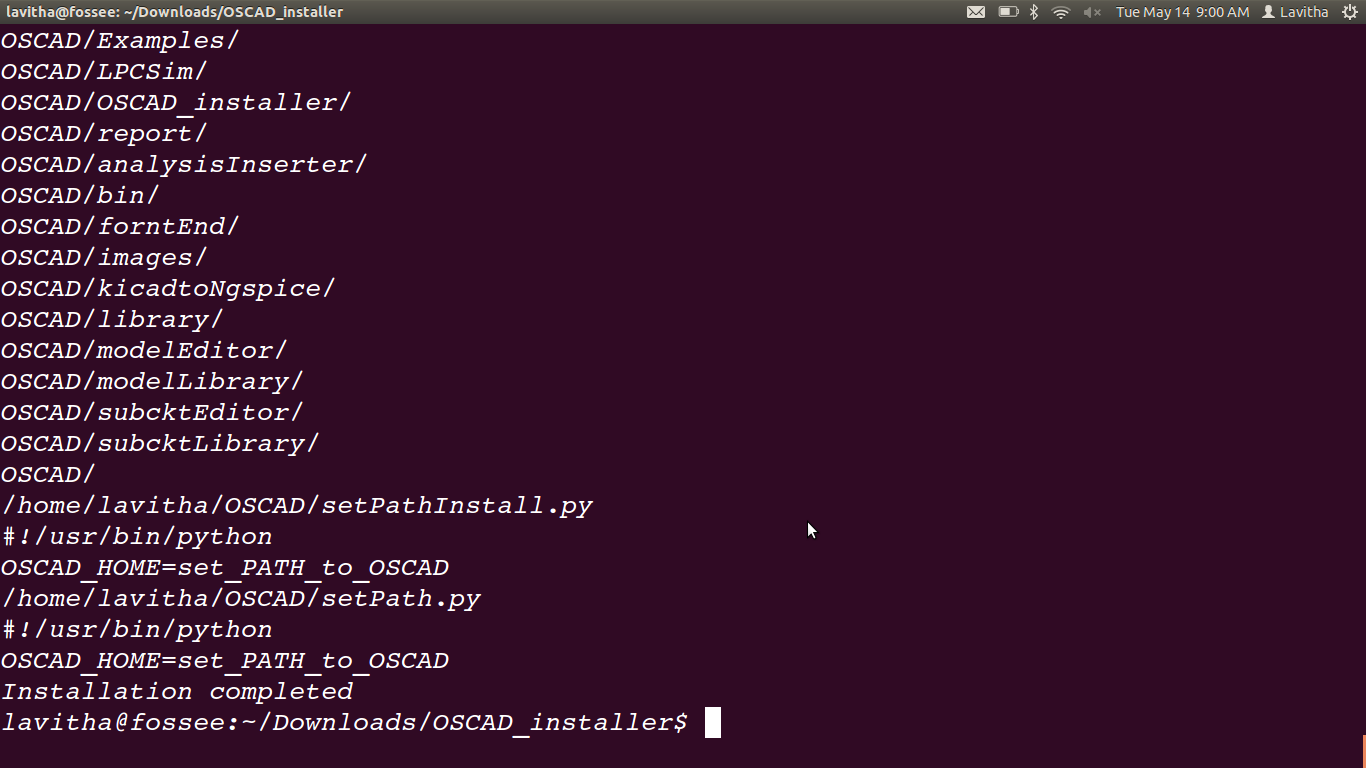
\includegraphics[width=0.9\textwidth]{figures/install9.png}
\caption{Terminal: Installation Completed}
\label{installi}
\end{figure}

%%%%%%%%%%%%%%%%%%%%%%%%%%%%%%%%%%%%%%%%%%%%%%%%%%%%%%%%%%%%%%%%%%%%%%%%%%%%%%%%%%%%%%%%%%%%%%%%%%%%%%%%%%%%%%%%%%%%%%%%%%%%%%%%%%%%%%%%%%%%%%%%%%%%%%%5
\section {Testing}
Let us now verify the installation of Oscad.
\begin{itemize}
\item Double click on Oscad shortcut created on Desktop as shown in figure \ref{osc}\\
\end{itemize}
\begin{figure}[h]
\centering
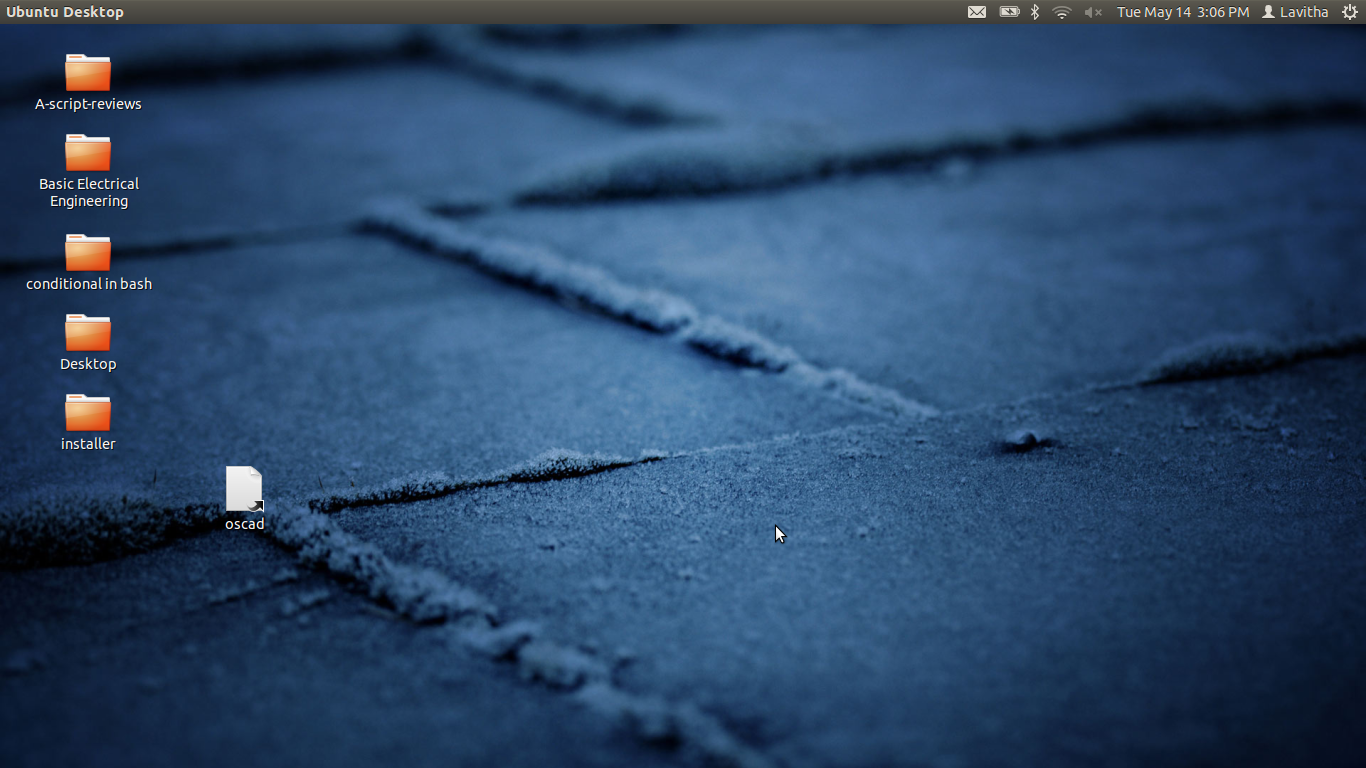
\includegraphics[width=0.9\textwidth]{figures/screenshot1.png}
\caption{Desktop: Oscad shortcut}
\label{osc}
\end{figure}
%%%%%%%%%%%%%%%%%%%%%%%%%%%%%%%%%%%%%%%%%%%%
\newpage
\begin{itemize}
\item A window is displayed as shown in figure \ref{tab}. Select the option \textbf{Run}\\
\end{itemize}
\begin{figure}[h]
\centering
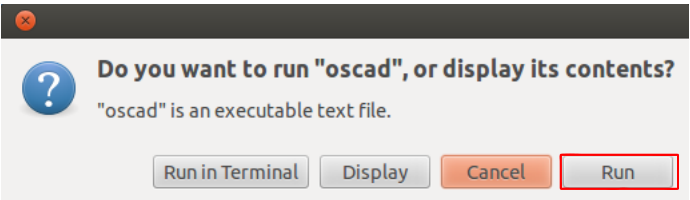
\includegraphics[width=0.9\textwidth]{figures/run.png}
\caption{Desktop: Oscad - Choose the option `run' }
\label{tab}
\end{figure}
%%%%%%%%%%%%%%%%%%%%%%%%%%%%%%%%%%%%%%%%%%%%%%%%%
\begin{itemize}
\item It opens the Oscad window as shown in figure \ref{window}
\end{itemize}
\begin{figure}[h]
\centering
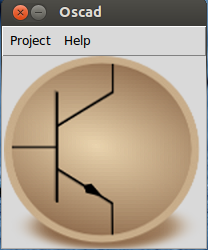
\includegraphics[width=0.2\textwidth]{figures/oscadicon.png}
\caption{Desktop: Oscad }
\label{window}
\end{figure}
\newpage
%%%%%%%%%%%%%%%%%%%%%%%%%%%%%%%%%%%%%%%%%%%%%
\newpage
\begin{itemize}
\item Select \textbf{project} tab at the top left hand corner of Oscad window and then click on \textbf{open}\\
Browse to the folder where Examples are saved as shown in figure \ref{Rc} 
\end{itemize}
\begin{figure}[h]
\centering
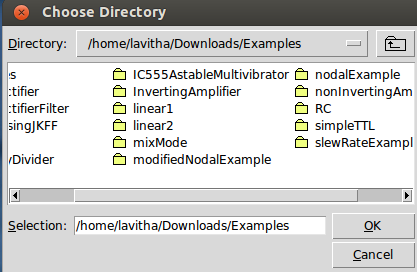
\includegraphics[width=0.9\textwidth]{figures/RC.png}
\caption{Browse to the folder where Oscad Examples are saved}
\label{Rc}
\end{figure}
%%%%%%%%%%%%%%%%%%%%%%%%%%%%
%%%%%%%%%%%%%%%%%%%%%%%%%%%%%
\begin{itemize}
\item Select \textbf{RC} from the examples by double clicking on RC and then click on \textbf{OK}
\end{itemize}
%%%%%%%%%%%%%%%%%%%%%%%%%%%%%%%%%%%%%%%%
\begin{itemize}
\item {\tt Enter Project name} dialog box opens up as shown in figure \ref{rcb}. Click on \textbf{OK}
\end{itemize}
\begin{figure}[h!]
\centering
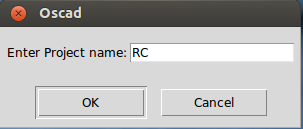
\includegraphics[width=0.6\textwidth]{figures/RC1.png}
\caption{Desktop: Oscad }
\label{rcb}
\end{figure}
%%%%%%%%%%%%%%%%%%%%%%%%%%%%%%%%%%%%%%%%%%%
\begin{itemize}
\item A tool bar appears as in figure \ref{tools}. Select \textbf{Schematic Editor} in the tool bar.
\end{itemize}
\begin{figure}[h]
\centering
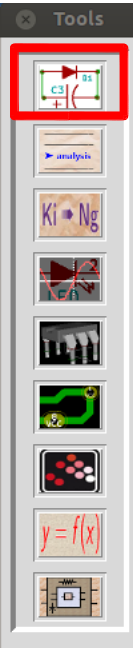
\includegraphics[width=0.1\textwidth]{figures/tools.png}
\caption{Desktop: Oscad Toolbar - Schematic editor}
\label{tools}
\end{figure}
%%%%%%%%%%%%%%%%%%%%%%%%%%%%%%%%%%%%%%%%%%%%
\begin{itemize}
\item An error message as shown in figure \ref{error} will pop up. Click on \textbf{Close}.
\end{itemize}
\begin{figure}[h]
\centering
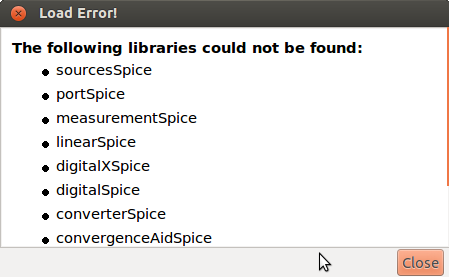
\includegraphics[width=0.5\textwidth]{figures/error.png}
\caption{Schematic editor Load error }.
\label{error}
\end{figure}
%%%%%%%%%%%%%%%%%%%%%%%%%%%%%%%%%%%%%%%%%%%%
\newpage
\begin{itemize}
\item Scematic Editor window appears. Press \textbf{F1} to zoom in and press \textbf{F2} to zoom out. RC filter circuit seen on schematic editor window is as shown in Figure \ref{schematic}.
\end{itemize}
\begin{figure}[h]
\centering
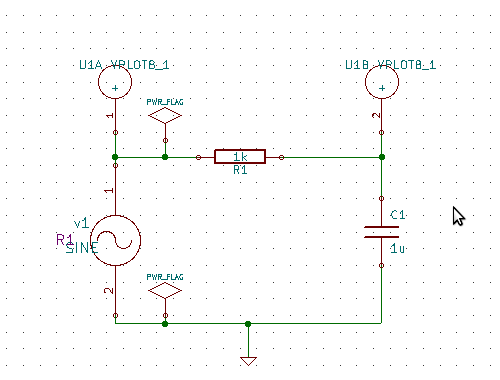
\includegraphics[width=0.5\textwidth]{figures/schematic.png}
\caption{Schematic of RC circuit }.
\label{schematic}
\end{figure}
%%%%%%%%%%%%%%%%%%%%%%%%%%%%%%%%%%%%%%%%%%%%%
\begin{itemize}
\item Close Schematic Editor
\end{itemize}
%%%%%%%%%%%%%%%%%%%%%%%%%%%
\begin{itemize}
\item Click on Ngspice from Oscad Tool bar as shown in Figure \ref{tools2}. This will simulate the netlist using Ngspice.\index{Netlist}
\end{itemize}
\begin{figure}[h]
\centering
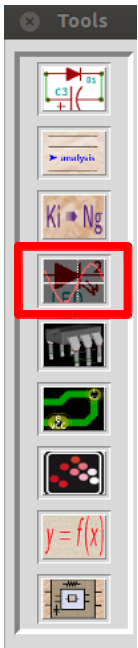
\includegraphics[width=0.1\textwidth]{figures/tools2.png}
\caption{Desktop: Oscad Toolbar - Ngspice }
\label{tools2}
\end{figure}
%%%%%%%%%%%%%%%%%%%%%%%%%%%
\begin{itemize}
\item The graph and terminal appears as shown in figure \ref{sch}. This shows the result of transient analysis of RC circuit and verifies installation.
\begin{figure}[h]
\centering
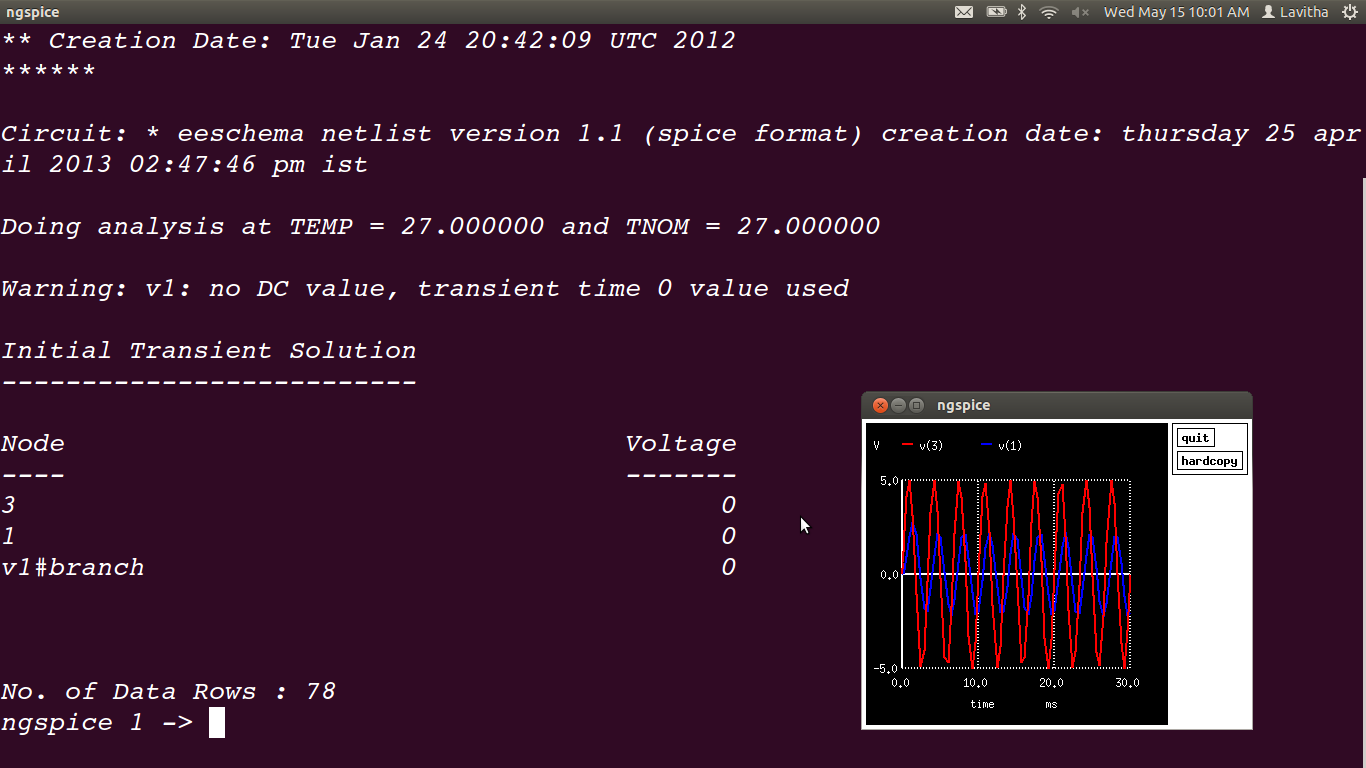
\includegraphics[width=1.2\textwidth]{figures/output.png}
\caption{Ngspice simulation output }.
\label{sch}
\end{figure}
\end{itemize}
%%%%%%%%%%%%%%%%%%%%%%%%%%%%%%

